\chapter{Conflicting Paradigms}
Numerous programming paradigms exist for even more general programming languages. Each of them come with different perks and offer different perspectives for a problem. Different programming paradigms, however don't necessarily exclude each other. Languages like \textit{Lisp} or \textit{Scala} for example both combine functional and object oriented programming.\\
This thesis will specifically concentrate on \textit{Object Oriented Programming} (OOP) and \textit{Data Oriented Design} (DoD). Whether or not data oriented design is even to be considered a programming paradigm is debatable \mcp{fabian}{TODO}, however its fundamental ideas (specifically concerning data layout) conflict with those of existing paradigms like OOP, so for the sake of consistency in this manner of comparison, we will call it that way.\\ 
Depending on the domain, certain programmers will have different answers to the question which of both should be preferred. Each party will make compelling arguments to why their choice is mandatory. This is because those paradigms (partially) solve different problems and therefore offer dissenting perspectives on problems and their respective solutions for them.
To understand why \textit{Object Oriented Programming} and \textit{Data Oriented Design} are rather cannibalistic to each other, we need to first have a look to what they are trying to solve, independently.

\section{Object Oriented Programming / AOS}
Starting with punch cards, each iteration of new programming generations provided new forms of abstraction for programmers, be it control flow statements, type systems, data structures like native arrays. When machine code started to simplify operations, FORTRAN partly introduced portability as early as 1957; LISP introduced symbolic processing and automated memory management until finally Simula/67 introduced objects in the 1960s \mc{louden}\mc{hopl}.
Object Oriented Programming could not be called popular until the 1970s or 1980s, when Stroustrup created C++. Originally OOP was meant to be the way to go for creating graphics based applications  \mc{about_oop}. This makes sense, since tree like data structures (GUIs), containing entities with shared behavior can easily be described through polymorphism.\\
OOP shines, whenever the problem to be modeled can be abstracted to one or more base classes, that define shared data and/or behavior. Even though some languages allow for a subclass to "\textit{exclude variables and/or methods which would otherwise have been inherited from the superclass(es)}" \mcp{what_is_oop}{4}.\\
OOP quickly established and rooted itself in the industry without solely being used on graphics applications. This is due to the fact, that it represents a world model, we are taught since elementary school. We are familiar with \textit{is-a} relations ever since we learned that despite dissenting traits, both Labradors and Pugs are dogs. Arguably abstraction is one of - if not - the most important disciplines in programming \mcp{ghezzi}{5}. Since programs oftentimes try to model real life information, OOP delivers an easy to grasp, quick-to-learn approach to do so. That is also the reason, why there are so many OOP programmers around the world. Without trying to evaluate whether or not OOP's way of abstraction is superior to DoD, it is undoubtedly the more prominent one, especially for virtually any other profession than a programmer/computer scientist \reffigp{lang_ratings}.
\begin{figure}[!htbp]
	\centering
	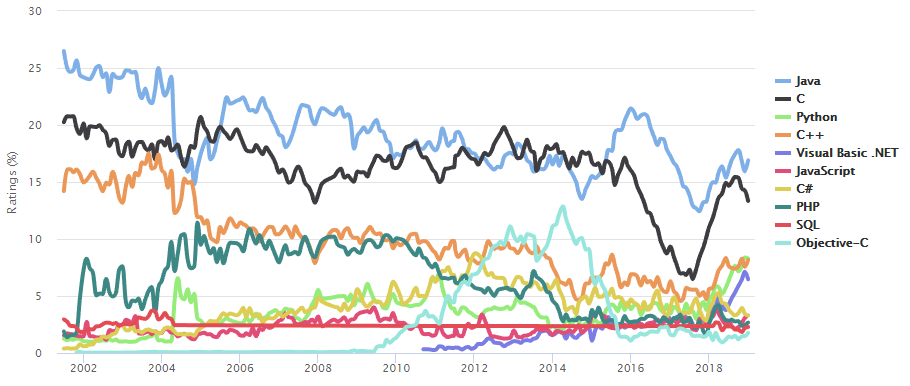
\includegraphics[width=1.0\linewidth]{PICs/lang_ratings}
	\caption{Most popular programming languages throughout the years \mcpic{lang_ratings}.}\label{lang_ratings}
\end{figure}
 This is however where OOP and modern computer architectures don't get along, so to say. OOP ovvers an elegant way to intuitively model an issue into code, but doing so it encourages us to implement our data in an inefficient way. Inefficient because creating monolithic models of our data usually lack cohesion, which means, that the classes' members tend to not be related/dependent \mc{cohesion} - at least in terms of computational order.\\
 In a home office application, juggling a few dozens of entities every other minute, this will not appear as a problem. And in this case it might be preferable to program such application in a strict object oriented way, since the development can be done fast and reliably even by a novice. On the other hand and especially in the game development industry OOP has proven to result in poorly performing software, due to inefficient data layouts. Because especially for games: data is performance \mcp{nystrom}{272}.\\
 The abbreviation \textit{AOS} stands for \textit{Array Of Structures}\mc{intel} and it describes, what usually happens with Object Oriented Programming.\\
 \begin{lstlisting}[language=C++,numbers=none,name={Example of some hierarchical POD class definitions},label={pods}]
struct Obj {				struct Human : Obj {			struct NPC : Human {
	float xyz[3];				char *name;						int mood;
	float vel[3];				int age;						};
};							};

NPC npc_arr[3];
 \end{lstlisting}
Considering the rather arbitrary C++ class definitions in \refcode{pods} the \textit{npc\_arr} will occupy memory according to \reffig{npcs_in_memory} (disregarding any \textit{padding}).
\begin{figure}[!htbp]
	\centering
	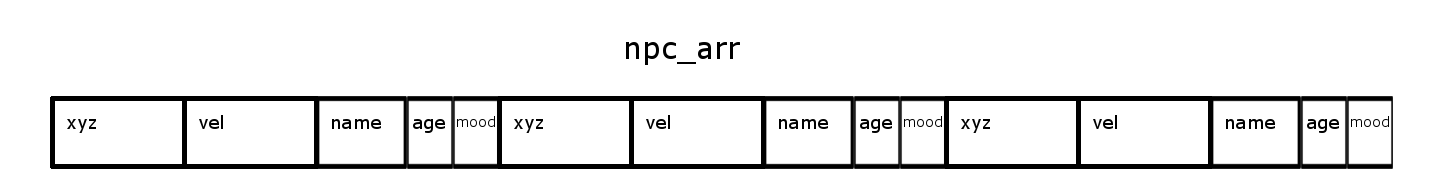
\includegraphics[width=1.0\linewidth]{PICs/npcs_in_memory}
	\caption{Visualization of how a \textit{npc\_arr} will exist in memory}\label{npcs_in_memory}
\end{figure}
This is quite literally an array of structures - hence the notation \textit{AOS}. The following sections \ref{cpu_caches} and \ref{dod} will elaborate on \textit{why} exactly this way of thinking/way of abstraction is inefficient.




\section{CPU Caches and why they don't \textit{fit} objects}\label{cpu_caches}
The data layouts typically found when programming with objects and classes, are not inefficient because they lack logic. "\textit{Each human - including students - will have positional traits}", is semantically correct. In fact it seems rather unfortunate, that modern computer architectures can't deal well with an abstraction that fits our perception of the world. But the hardware is certainly not to blame here. The problem with a monolithic class definition is much more that of common coding- or data access patterns.\\
\subsection{Common data access patterns vs. Monolithic class definitions}\label{cdap}

Numerous coding best practices teach us to write simple, modular code.
\begin{quote}
	\textit{Functions should do one thing. They should do it well. They should do it only.} \mcp{rcmartin}{35}
	
	\textit{Keep it simple and smart} (KISS principle). \mcp{niemann_kiss}{77}
	
	\textit{[...] cohesion is an important object-oriented
		software quality attribute.}\mc{cohesion}
\end{quote}
Just like we want our class definitions to share a common responsibility or task, we want the set of instructions that iterate and probably transform a set of data to be as simple and modular as possible. So usually we try to not write monolithic \textit{for-loops} handling every single aspect of a set of data.\\ For example in \reffig{npcs_in_memory} we would not want a loop that handles each and every single member of an NPC. This would not only result in a big set of instructions, that hide the individual purposes of each expression, but also make it hard to maintain/change the code. Not to mention, that different data often demands change at different times at runtime. Requirements can change quickly. Breaking up responsibilities that were coupled and forced to coexist change not so quickly.\mc{rcmartin}\\
Exemplary if \refcode{pods} was the model for a game, our game loop could at one point iterate over all the elements in the \textit{npc\_arr} to update their position and velocity for each frame. The \textit{NPC's mood} could just as well be updated frequently in a separate function, that only encompasses the information relevant for the calculation of the updated mood.
Their \textit{Human::name}s however will most likely not change so frequently - if ever - so the instructions to modify that data will most likely depend on user input and exist in yet a whole other routine. This modularization of code is commonly referred to as \textit{Separation of Concern} and has proven to improve the code's maintainability \mcp{laplante}{85}.
\textit{This} keeping the objects in some sort of set, then iterating over it for each routine, that manages a subset of the object's data, is a common access pattern that is applied on objects in OOP.\\
The interim conclusion here is, that even only for maintainability reasons, it is desirable for programmers to process logically related subsets of their data separately - but then why is the resulting software so slow compared to the same idea implemented with a \textit{Data oriented Design}?\\
The Object Oriented Programming paradigm is exactly doing what it promises - providing a sort of abstraction, that programmers can intuitively apply to their problem definition. Consequently OOP programmers quickly adapt the habit of developing against their abstraction because it is intuitive. What is lost in the process is the concern of developing against the hardware. \textit{This} is probably the fundamental difference between OOP and DoD.\\
So whats our hardware's deal? Why do objects don't get along with it. Why can't we have super high speed machinery, that makes hardware concerns obsolete? Why can't we have anything nice?

\subsection{A brief history of memory}
To answer \refsec{cdap}'s concluding question: We do have high speed memory units at hand we just can't afford them. Modern computer systems rely on a variety of different memory units each differing in access latency and other properties. The intention behind this complex hierarchy of memory layers is obviously speed and is the result of an evolving cost-benefit calculation.
\begin{quote}
	\textit{The task the computer designer faces is [...] design a computer to maximize
		performance while staying within cost[...].}\mcp{hennessy}{8}
\end{quote}

Originally
\begin{quote}
	\textit{memory access latency and instruction execution latency were on roughly equal footing. [...] register-based instructions could execute in two to four cycles, and a main memory access also took roughly four cycles.}\mcp{gregory}{189}
\end{quote}
This proportion changed significantly. While it is relatively cheap to produce high speed CPUs the same is not true for memory units. So whats happening, is that today's PCs/consoles are equipped with CPUs that are way faster than the greater parts of their available memory units. Due to increasing tick rates and \textit{Instruction Pipelining} what used to be ~four cycle RAM reads are now several hundred cycles. Not Because RAM became slower - the opposite is the case - but because CPUs became that much faster in relation.
This trend was thoroughly observed and documented by John L. Hennessy and David A. Patterson \reffigp{cpu_memory_gap}.\\
\begin{figure}[!htbp]
	\centering
	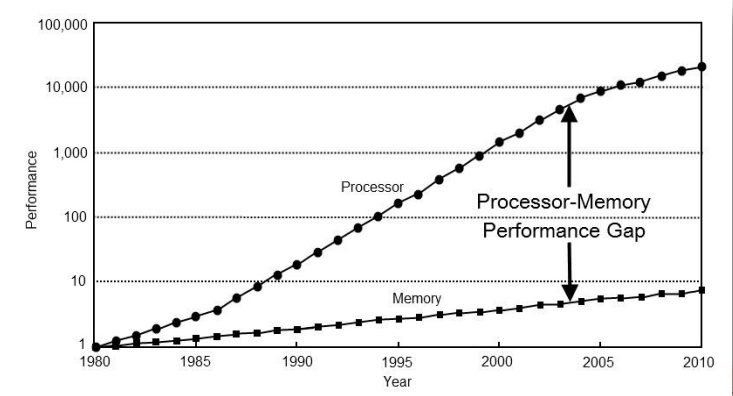
\includegraphics[width=0.7\linewidth]{PICs/cpu_memory_gap}
	\caption{"\textit{\textbf{Starting with 1980 performance as a baseline, the gap in performance
			between memory and processors is plotted over time}.
			Note that the vertical axis
			must be on a logarithmic scale to record the size of the processor-DRAM performance
			gap. The memory baseline is 64 KB DRAM in 1980, with a 1.07 per year performance
			improvement in latency (see Figure 5.13 on page 313). The processor line assumes a
			1.25 improvement per year until 1986, and a 1.52 improvement until 2004, and a 1.20
			improvement thereafter}" \mcppic{hennessy}{289}}\label{cpu_memory_gap}
\end{figure}\\
To solve the issue of ever diverging CPU/memory performances (commonly referred to as the \textit{memory gap \mc{gregory}}), specifically to reduce the latency of references to main memory, smaller but significantly faster (and more expensive) memory units are placed between the CPU and the main memory. These modules are called \textit{Caches} - first named by C.J. Conti \mc{conti} in 1969. Originally cache technology was mentioned as \textit{buffers}\mc{cragon}. Not considering their complex, modern modalities and policies this is a fitting notation.\\
The basic idea behind a fast buffer interconnected between the CPU and the main memory is to create local copies of referenced data-chunks, in order to provide faster access on subsequent calls to the same \textit{AU} (Adressable Unit) as well as the ones deemed likely to be accessed soon \mcp{gregory}{191}. This principle originated in the work on \textit{Virtual Memory} \mcp{cragon}{15} and is today much more sophisticated.\\
So we actually do use high speed memory in our common computer architecture, we just don't have lots of it.

\subsection{Cache modules and types}
In today's PCs/consoles typically each CPU core has its own hierarchy of cache modules \reffigp{cache_layout}.
\begin{figure}[!htbp]
	\centering
	\includegraphics[width=0.4\linewidth]{PICs/cachelayout}
	\caption{Exemplary, simplified model of a CPU core and its several cache modules \mcppic{Drepper}{15}}\label{cache_layout}
\end{figure}
Closest to the core (on-chip) is the \textit{L1} (Level 1) cache. Accessing an AU in the  Intel® Core™ i7 Processor's L1 cache for example is almost as fast as accessing it in the very CPU's register - ~4 cycles (2.1 to 1.2 ns) \mc{levinthal}. For reference access to main RAM "\textit{can take on the order of 500 cycles[...]"} \mcp{gregory}{189}.
Another cost unrelated reason, why we don't have lots of \textit{L1 D} cache is that more memory literally means more physical space is occupied. Having more cache memory equals more \textit{cache hits} \refsecp{cpucu} but as soon as the cache won't fit on-chip anymore, there is yet again additional latency. Thats why the L1 and sometimes L2 cache modules are kept comparably small but on-chip. Other L3 and L4 caches are each bigger and slower than their preceding counterparts respectively, but for the most part share the same ideas slowly converging latency times to the common main memory RAM.\\
CPU cores can share one or more cache modules (usually starting with L2 or L3), effectively accessing the same local copies. This entails synchronization issues, that will be mentioned in the context of this work later on (TODO).\\
Modern cache hierarchies include data caches as well as instruction caches, usually both in an L1 cache. However there are different takes on how to implement this. Harvey G. Cragon lists \mcp{cragon}{17}:
\begin{itemize}
	\item instruction cache - holds only instructions
	\item data cache - holds only the data stream
	\item unified cache - holds both instructions and data
	\item split cache - two-cache system, one for instructions and one for data
\end{itemize}
The scope of this masters thesis will omit instruction-cache related subjects, because the upcoming attempts and techniques to achieve performance optimizations will focus on improving the data layout of a given target source code.
%local  L1 CACHE hit,                              ~4 cycles (   2.1 -  1.2 ns )
%local  L2 CACHE hit,                             ~10 cycles (   5.3 -  3.0 ns )
%local  L3 CACHE hit, line unshared               ~40 cycles (  21.4 - 12.0 ns )
%local  L3 CACHE hit, shared line in another core ~65 cycles (  34.8 - 19.5 ns )
%local  L3 CACHE hit, modified in another core    ~75 cycles (  40.2 - 22.5 ns )
%remote L3 CACHE (Ref: Fig.1 [Pg. 5])        ~100-300 cycles ( 160.7 - 30.0 ns )

\subsection{The CPUs cache utilization}\label{cpucu}
A programmer will rarely ever directly interact with a cache module (though there are mechanisms for manual prefetching/clearing). The underlying idea for it was to be transparent to the programmer. However understanding the CPUs cache utilization enables one to tailor the data layout to it, resulting in faster access, less waiting and consequently higher throughput. This is what \textit{Data oriented Design} aims to do - because it develops against hardware concerns.\\
As mentioned before the basic idea of the cache is to provide local copies of data at a faster rate and prefetch data segments, that are likely to be used soon. This works by directing each main memory access to go through the cache. Main memory access means also going through virtual address translation, address and data buses and depending on the main memory crossbar switching logic \mcp{gregory}{190}.  
Whenever the CPU requests access to a certain AU before saddling the horses and going on a journey to main memory, the cache will check whether or not the requested AU is currently present inside its buffer. If so it is referred to as a \textit{cache hit}, otherwise a \textit{cache miss}. For a modern L1 D cache this buffer, to be more specific, consists of several cache lines each of 64 bytes. Overall cache- and line sizes vary between different architectures but are standardized mostly due to Intel's work.\\
The simplest and least efficient implementation to determine a cache \textit{hit/miss} is to iterate each cache line comparing fitting criteria. To prevent this nowadays caches implement a certain associativity technique. This way each individual physical main memory address can be mapped to one or more specific cache lines. Doing so addresses are converted to and managed by metadata  consisting of: \mcp{gregory}{193}
\begin{itemize}
	\item Offset - Offset to the actual referenced Byte inside the cache line.
	\item Cache Line Index - Which cache line/s would hold the AU.
	\item Tag - Which cache sized block in main memory holds the original data.
\end{itemize}
In the case that each physical main memory address, has exactly one counterpart it is called a \textit{direct-mapped} cache \mcp{gregory}{194}. In this case since the cache can by far not encompass the whole extend of the main memory, a lot of physical addresses will be mapped to the very same cache line, effectively extruding each other out of the cache. This is called \textit{eviction} and in unlucky cases will behave like all references are cache misses \mcp{cragon}{97}. To prevent this modern caches map a physical address to \textit{n} cache lines. This is called \textit{n-way associativity} - typically implemented as \textit{8-way} or \textit{16-way} caches depending on the level.\\
There is a lot more to cover about caching technologies and policies like: Replacement-/Write-/Coherency(MESI; MOESI; MESIF) policies and for further reading Harvey G. Cragon's \textit{Memory Systems and Pipelined Processors}\mc{cragon} as well as Jason Gregory's \textit{Game Engine Architecture}\mc{gregory} are highly recommended reads. However for the purpose of this work a few specifics are most interesting for us.\\
How can a data layout affect \textit{hit ratios} and reduce calls to main memory? As mentioned before there are common data access patterns in software and the caches actually accommodate us by adapting their builtin prefetching mechanisms to it, following a set of \textit{locality concepts}. Harvey G. Cragon counts three of those concepts: \mcp{cragon}{16}
\begin{itemize}
	\item \textit{Temporal locality} - Information recently referenced by a program is likely to be used again soon.
	\item \textit{Spatial locality} - Portions of the address space near the current locus of reference are likely to be referenced in the near future.
	\item \textit{Sequential locality} - A special case of spatial locality in which the address of the next will be the immediate successor of the present one.
\end{itemize}
At first glance these concepts are very straight forward, but their respective implementation for automatic hardware prefetching is more complex than one would think. Prefetching basically means:
\begin{quote}
"\textit{[...] bringing data in the data (or mixed instruction-data) cache before it is directly accessed by a memory instruction [...].}" \mcp{chen}{610}
\end{quote}
There are however different strategies to decide which bytes should be faithfully loaded into the cache. Tien-Fu Chen and Jean-Loup Baer list two categories for prefetching strategies: \mcp{chen}{610}
\begin{itemize}
	\item \textit{Spatial} - access to current block is basis for prefetching.
	\item \textit{Temporal} - lookahead decoding of instruction stream is implied.
\end{itemize}
There are simple approaches like: whenever block \textit{i} is accessed, prefetch block \textit{i}+1, called the \textit{One Block Lookahead}; stride based approaches storing previously referenced addresses in a table and calculating a stride based on current and previous addresses; combinations of both and many more \mc{chen}.  Sometimes data is prefetched into the cache, sometimes into separate stream buffers. There are many different hardware prefetching methods to find and while data cache prefetching is considered to be more challanging \mcp{mittal}{4} it is still best practice to rely on spatial locality when modeling data to play into the cache's hand.\\
Compilers already make use of software prefetching in certain cases.
\begin{quote}
	\textit{For array-based applications, the compiler can use locality analysis to predict which dynamic references to prefetch, and loop splitting and software pipelining to schedule prefetches.} \mcp{luk}{223}
\end{quote}
So we can already deduce that for an efficient data layout it would be beneficial to rely on arrays, or more generally, concepts compilers can 'comprehend' and optimize. Also even though the concept of \textit{sequential locality} is only a special case, it is the one we can utilize best to derive adaptations for our data layout, since hardware prefetching has adapted best to it. How exactly can we convert this information into a generic set of rules/best practices, a manifesto of efficiency? We don't it already exists.

\section{Data Oriented Design / SOA}\label{dod}
